\documentclass[
    12pt, % Schriftgröße
    oneside, % zweiseitiger Modus
    ngerman, % deutsches Dokument
    BCOR=0mm, % Bindungskorrektur
    DIV=10 % Division (Anzahl Spalten/Zeilen pro Seite, bestimmt implizit Margins)
]{scrreprt}

\newcommand{\titleDocument}{Dokumentation der Praktischen Arbeit zur Prüfung zum Mathematisch-technischen Softwareentwickler}
\newcommand{\authorDocument}{Natalie Fritzen}
\newcommand{\subjectDocument}{Großprogrammierung}
\newcommand{\locationDocument}{Köln}
\newcommand{\dateDocument}{\today}

\title{\titleDocument}
\author{\authorDocument}
\date{\dateDocument}

%Style importieren:
\usepackage{dokumentation}
\usepackage[nofiller, verification]{struktex}

\begin{document}
    % ============ Anfang =============
    % Titelseite
    \begin{titlepage}
	% TODO: wird das geometry Paket genutzt statt der Mechanismen aus KOMA-Skript, kann die folgende Zeile z.B. durch "\newgeometry{...}" ersetzt werden
	\typearea{100} % DVI auf 100 setzen für Titel (kleine Margins)
	\setlength{\parindent}{0pt} % keine Einrückung bei neuen Absätzen auf dieser Seite

	\begin{flushright}
		\includegraphics[height=5cm]{images/FH-Aachen-r_svg-raw}
	\end{flushright}
	
	\vspace*{-2.5cm}

	\begin{center}
		\textbf{\Huge Fachhochschule~Aachen}

		\vspace*{0.5cm}
		
		\textbf{\Huge Studienort Köln}

		\vspace*{0.75cm}

		{\normalsize\doublespacing Fachbereich~9:~Medizintechnik~und~Technomathematik\\	Studiengang:~Angewandte~Mathematik~und~Informatik}

		\vspace*{2.5cm} % TODO: bei mehr verwendeten Zeilen für den Titel verringern
		
		\begin{minipage}[t]{14cm} % TODO: abhängig von dem konkreten Titel muss diese Breite eventuell angepasst werden für einen passenden Zeilenumbruch
			\begin{center}
				\textbf{\Huge \titleDocument}
			\end{center}
		\end{minipage}
	
		\vspace*{2.5cm} % TODO: bei mehr verwendeten Zeilen für den Titel verringern (symmetrisch zu oben)
		
		\textbf{\Large \subjectDocument}

		\vspace*{0.5cm}
		
		{\normalsize von}
		
		\vspace*{0.5cm}
		
		\textbf{\Large \authorDocument}
	
		\vspace*{3.5cm}
		
		\begin{minipage}[t]{13cm}
			\begin{center}
				\begin{tabular}{llll}
					Matrikelnummern: & 3240219 \\
				\end{tabular}
			\end{center}
		\end{minipage}
		
		\vspace*{2.5cm}
	
		{\large \locationDocument, den \dateDocument}
	\end{center}
\end{titlepage}


    \tableofcontents

    % =========== Zahlenteil ===========
    \chapter{Aufgabenanalyse}\label{ch:aufgabenanalyse}


\section{Interpretation der Aufgabe}\label{sec:interpretation-der-aufgabe}
Im Flächengebiet der Matsedanier sollen Antennen aufgestellt werden, sodass jeder Eckpunkt der Teilflächen erreicht wird, da davon ausgegangen wird, wenn die Eckpunkte erreicht werden, wird die komplette Teilfläche erreicht.
Um so wenig wie mögliche Antennen aufzustellen, soll ein Programm entwickelt werden, welches überprüft, wie viele minimal aufgestellt werden müssen.
Hierfür wird überprüft, dass eine Antenne möglichst viele Punkte erreicht und dabei keine andere Fläche durchdringt.
\\
Das Programm arbeitet hierfür mit dem Eingabe-Verarbeitung-Ausgabe-Prinzip.
Zunächst werden die Daten für das Flächengebiet eingelesen.
Die Datei enthält den Namen des Beispiels, die Größen des zu berechnenden Bereiches und die Höhenangaben an den Eckpunkten.
Es muss mindestens eine Angabe für die Höhe in der Zeile sein, da dann von ausgegangen wird, dass die nachfolgenden Höhen der vorangestellten entsprechen.
Nachdem das Programm die Mindestanzahl an Antennen berechnet hat, werden mindestens vier Ausgabedateien erzeugt.
Die Erste enthält die Eingabewerte, die Antennenanzahl und die Koordinaten der einzelnen Antennen.
Die Zweite enthält die Anweisungen für GnuPlot, die Dritte enthält die Eckpunktkoordinaten der Teilflächen und die Vierte und Folgenden enthalten die Koordinaten der Antennen.
\\
Im Programm werden die eingelesenen Daten in einer Klasse Punkt gespeichert, diese enthält die drei Koordinaten des Eckpunktes.
Im Vergleich zur Überlegung an Tag 1 ergibt diese Art des Speicherns der Daten den Vorteil, die Daten gekapselt zu nutzen und sortiert zu speichern.
Hierbei sind die Koordinaten als Double gespeichert, obwohl die Koordinaten keine Nachkommastellen besitzen, da die Schnittpunkte bei der Berechnung der Erreichbarkeit Nachkommastellen besitzen können.
\\
Beim Einlesen werden die Daten überprüft, unter anderem wird die Anzahl der Daten überprüft, ob diese der Größe des Feldes entsprechen.
Wenn die x-Koordinaten-Anzahl nicht mit der angegebenen Größe übereinstimmt, werden diese mit dem letzten Wert aufgefüllt.
Falls die y-Koordinaten-Anzahl nicht übereinstimmt, wird abgebrochen und eine Exception geworfen.
\\
Der Algorithmus, der am ersten Tag beschrieben wurde, war schwer als Programm umzusetzen, sodass ein neuer Algorithmus entwickelt wurde.
Der neue Algorithmus überprüft jede Möglichkeit eine einzelne Antenne aufzustellen, sodass jeder andere Punkt erreicht werden kann.
Hierbei startet die Überprüfung der möglichen Positionen bei dem höchstmöglichen Punkt und geht die Liste der Datenpunkte absteigend der Höhen entlang.
Falls nicht alle Punkte erreicht werden können, werden alle Möglichkeiten zwei Antennen aufzustellen überprüft.
Hierbei werden die Datenpunkte wieder absteigend der Höhen kombiniert.
Der Algorithmus überprüft danach jede Dreier-Kombinationen, Vierer usw.
Hierbei auch wieder der Höhe absteigend nach sortiert.
Der Algorithmus bricht ab, sobald alle Datenpunkte durch eine Antenne abgedeckt sind.
\\
Die Ausgabe passiert, nachdem die kleinste Anzahl an Antennen gefunden wurde.
Zunächst werden in der Konsole die Eingabedaten wiederholt und das Ergebnis der Antennenanzahl mit den Koordinaten aufgelistet.
Die erste Datei, die erzeugt wird, enthält ebenfalls diese Daten, die ausgegeben wurden.
Danach werden die Dateien für GnuPlot erzeugt.
Die erste Datei enthält die Anweisungen, um das Koordinatenfeld, die Felderflächen und Antennen zu setzen.
Die nächste Datei enthält die Koordinaten, die die Eckpunkte beschreiben.
Nachfolgend werden die Dateien für die Koordinaten der Antennen erzeugt.
Pro Datei werden die Koordinaten angegeben, die die Antennen aufspannen, da diese 10 Meter hoch ist.



\section{Fehlerarten}\label{sec:fehlerarten}

\subsection{Technische Fehler}\label{subsec:technische-fehler}
Ein technischer Fehler in dieser Software tritt auf, falls die einzulesende Datei nicht gefunden werden kann.
Das tritt auf, falls die Datei im falschen Ordner liegt und/oder nicht der gesamte Pfad zu dieser Datei eingegeben wird.

\subsection{Syntaktische Fehler}\label{subsec:syntaktische-fehler}
Beim Einlesen der Datei können viele Fehler auftreten.
Die Datei muss mindestens sieben Zeilen enthalten.
Hierbei werden die Kommentarzeilen mit gezählt und geprüft.
Die erste Zeile der Datei muss eine Kommentarzeile sein, also mit einem Semikolon starten.
Des Weiteren muss die erste Zeile "*" beinhalten.
Die zweite Zeile ist eine Kommentarzeile, die den Titel des Beispiels enthält.
Die dritte Zeile wird wie die erste überprüft.
Nachfolgend wird die nächste Zeile geprüft, dass diese wieder eine Kommentarzeile ist.
Die sechste Zeile muss auch eine Kommentarzeile sein.
Als Nächstes wird die Dimension in y-Richtung überprüft, ob diese der angegebenen Dimension entspricht.
Hierbei werden die Zeilen nach der letzten Kommentarzeile gezählt und mit der angegebenen Größe des Feldes verglichen.
Die Höhen und Dimensionen, die angegeben werden, dürfen keine Nachkommastellen haben.
Beim Schreiben der Ausgabe, kann es passieren, dass die Daten nicht in die Dateien geschrieben werden können.

\subsection{Semantische Fehler}\label{subsec:semantische-fehler}
In der fünften Zeile sollen die Dimensionen des gesamten Feldes angegeben werden, falls diese negativ oder null sind, tritt ein Fehler auf.
Des Weiteren dürfen angegebenen Höhen nur zwischen null und sechs gesetzt sein.

\section{Fehlerbehandlung}\label{sec:fehlerbehandlung}

\subsection{Technische Fehler}\label{subsec:technische-fehler-behandlung}
Das Programm bricht ab und kann mit dem richtigen Dateipfad/-namen neu gestartet werden.

\subsection{Syntaktische Fehler}\label{subsec:syntaktische-fehler-behandlung}
Jeder syntaktische Fehler hat seine eigene Fehlernachricht, die an den Nutzer weitergegeben wird.
Das Programm bricht ab.

\subsection{Semantische Fehler}\label{subsec:semantische-fehler-behandlung}
Es werden auch bei semantischen Fehlern Nachrichten an den Nutzer zurückgegeben und das Programm beendet sich.

\subsection{Sonderfälle}\label{subsec:sonderfaelle}
Wenn die Anzahl pro Zeile nicht mit der angegebenen x-Dimension des Feldes überein stimmt, werden die Werte mt dem letzten Wert aufgefüllt.

    \chapter{Verfahrensbeschreibung}\label{ch:verfahrensbeschreibung}

\section{Gesamtsystem}\label{sec:gesamtsystem}
Die entwickelte Software liest die Daten ein und führt die Prüfungen nach semantischen und syntaktischen Fehlern aus.
Danach ermittelt der Algorithmus die minimale Anzahl an Antennen, die benötigt wird, um alle Eckpunkte jeder Teilfläche zu erreichen.
Im Anschluss werden die Daten in der Konsole wiedergegeben und in eine Datei geschrieben, sowie die Anweisungen für GnuPlot geschrieben.

\subsection{Eingabe}\label{subsec:eingabe}
Beim Einlesen wird der Pfad, der eingegeben wird, genutzt und die Datei gelesen.
Nach allen syntaktischen und semantischen Überprüfungen werden die Variablen mit den Daten gefüllt.
Hierbei wird für jeden Höhenwert ein Punkt erstellt, der die x-, y- und z-Koordinate füllt.

\subsection{Verarbeitung}\label{subsec:verarbeitung}
Die Verarbeitung enthält den Algorithmus, der in mehrere Schritte aufgeteilt ist und dementsprechend unterschiedliche Methoden nutzt.
Der Algorithmus startet mit einer Antenne un prüft, ob es einen Punkt gibt, der alle anderen Punkte erreicht.
Danach werden alle Kombinationen errechnet, die zwei Antennen enthalten.
Diese Möglichkeiten werden iteriert und geschaut, ob mit dieser Kombination alle Eckpunkte erreichbar sind.
Wenn immer noch nicht alle Punkte erreicht wurden, werden drei Antennen gesetzt.
Dieses Verfahren nimmt nach jeder Iteration eine weitere Antenne dazu.
Sobald eine Möglichkeit gefunden wurde, alle Punkte zu erreichen, ist das die minimale Anzahl an Antennen.

\subsection{Ausgabe}\label{subsec:ausgabe}
Die Ausgabe erfolgt, sobald die Anzahl an Antennen gefunden wurde.
Zunächst werden die Eingabedaten wiederholt und die Antennenanzahl mit ihren Koordinaten in die Konsole ausgegeben und in eine Datei geschrieben.
Danach werden die Anweisungen für GnuPlot zusammengesetzt.
Für GnuPlot werden weitere Dateien benötigt, die die Koordinaten der Eckpunkte der Teilflächen enthält und jeweils eine Datei mit Koordinaten für jede Antennen.

\subsection{Datenstrukturen}\label{subsec:datenstrukt}
Innerhalb des Programms sind mehrere Modelle erstellt, um die Daten zu speichern und die Berechnung zu ermöglichen.
Das erste Modell Punkt hält die Koordinaten der einzelnen Höhen mit x- und y-Koordinate.
Außerdem enthält dieses Modell Methoden, um die Erreichbarkeit zwischen zwei Punkten zu prüfen.
Des Weiteren wird diese Klasse genutzt, um das nächste Modell aufzustellen.
Das Modell Gerade enthält zwei Vektoren, die als Punkt gespeichert werden.
Die beiden Punkte entsprechen dem Stütz- und Richtungsvektor, die eine Gerade im dreidimensionalen System aufspannen.
Das dritte genutzte Modell ist die Klasse Ebene, diese wird aus drei Vektoren erzeugt.
Hierbei ist der erste Punkt der Aufpunkt, bei dem die Ebene ansetzt.
Der zweite und dritte Punkt wird genutzt, um die Richtungsvektoren zu berechnen.
Die Logik des Algorithmus liegt im Controller Antennenminimum.
Die dritte Schicht des MVC-Systems ist View, die vom Nutzer den Pfad übergeben bekommt.
    \chapter{Programmbeschreibung}\label{ch:programmbeschreibung}


\section{Programmablaufplan}\label{sec:pap}

\begin{figure}
    \centering
    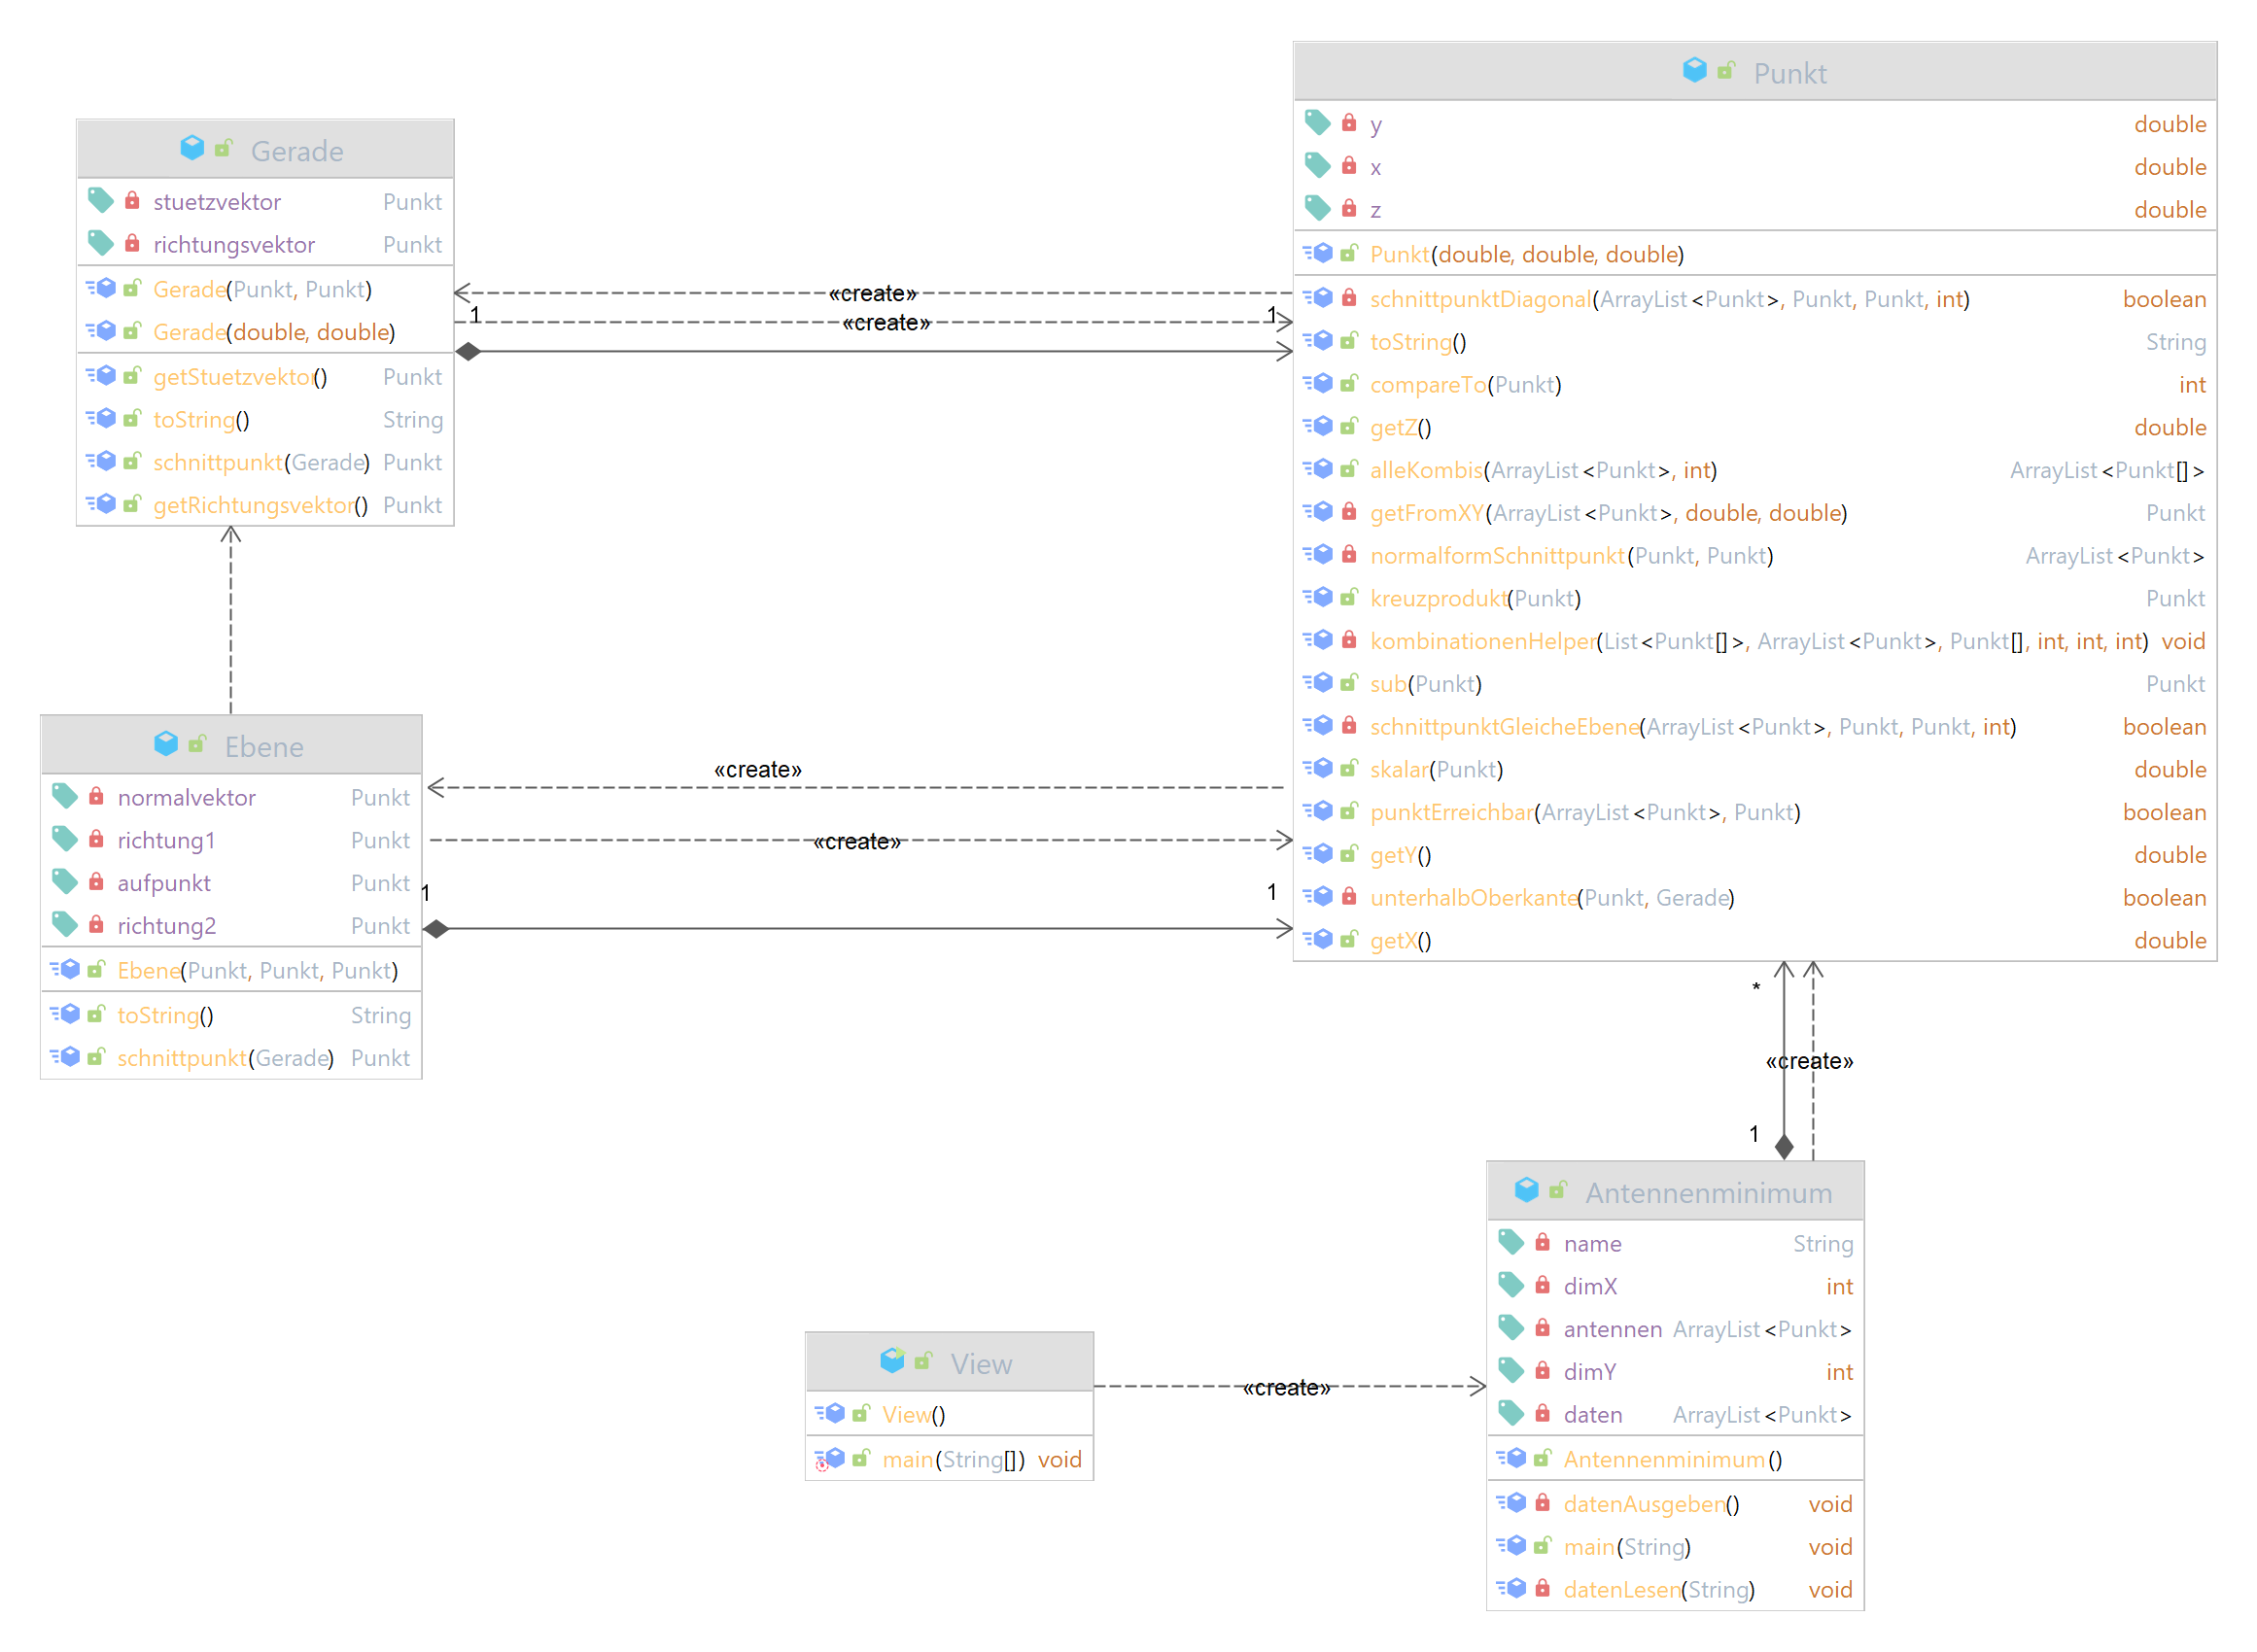
\includegraphics[scale=0.9,width=\textwidth,height=\textheight,keepaspectratio]{class-diagramm-light}
    \caption{Klassendiagramm}
    \label{fig:diagramm1}
\end{figure}

\begin{figure}
    \centering
    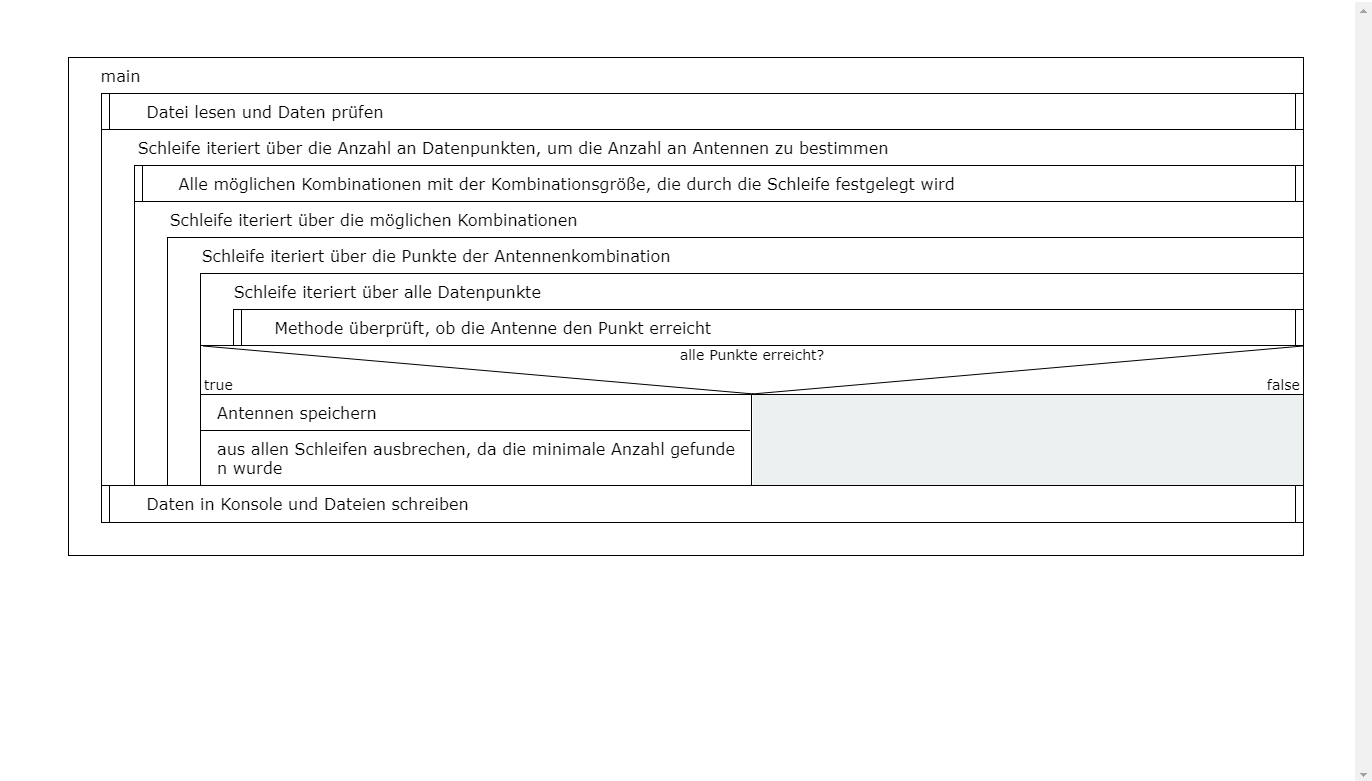
\includegraphics[scale=0.9,width=\textwidth,height=\textheight,keepaspectratio]{struktogramm-main}
    \caption{Struktogramm des Algorithmus}
    \label{fig:diagramm2}
\end{figure}

\begin{figure}[htb]
    \centering
    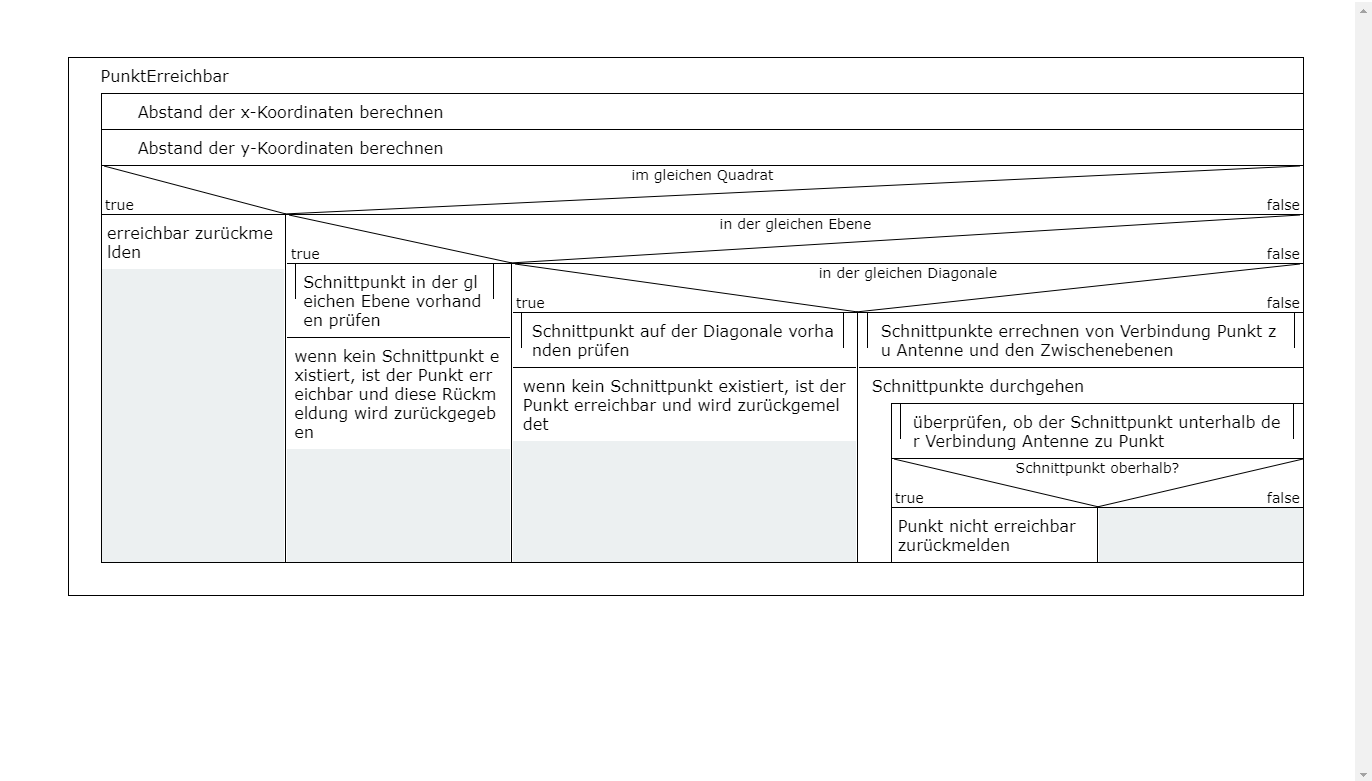
\includegraphics[scale=0.9,width=\textwidth,height=\textheight,keepaspectratio]{struktogramm-punktErreichbar}
    \caption{Struktogramm zur Methode Punkterreichbarkeit prüfen (if-else-Kaskade in Software nicht richtig darstellbar)}
    \label{fig:diagramm3}
\end{figure}



\section{Entwicklungsdokumentation}\label{sec:entwicklerdokumentation}
Im beigefügten Ordner "JavaDoc" ist eine generierte Dokumentation der Methoden zu finden.
\\
Näher zu beschreiben ist die Methode, die überprüft, ob ein Punkt durch eine Antenne erreichbar ist.
Hierbei wird unterteilt in mehrere Bedingung(siehe Struktogramm), zunächst wird geschaut, ob der Punkt im gleichen Quadrat wie die Antenne ist, also direkter Nachbar nach links, rechts, oben, unten oder diagonal ist.
Wenn der Punkt und die Antenne direkte Nachbarn sind, ist der Punkt erreichbar.
Danach wird die Ebene überprüft, das heißt es wird geschaut, ob der Punkt die gleiche x- oder y-Koordinate besitzt.
Dementsprechend wird die Erreichbarkeit geprüft.
Als Nächstes wird geschaut, ob der Punkt in einer direkten Diagonalen zu der Antenne liegt und hierbei auch die Erreichbarkeit.
Wenn diese Bedingungen alle nicht erfüllt werden, wird die letzte Methode aufgerufen, die zu jeder Zwischenebene einen Schnittpunkt errechnet und die Höhe mit der aktuellen Höhe der Verbindung vergleicht.


    \chapter{Testdokumentation}\label{ch:testdokumentation}
Aufgrund von Zeitmangel habe ich in der Simulation keine Testskripte oder Junit-Tests geschrieben.
Daher existiert

\section{Normalfälle}\label{sec:normalfaelle}
\section{Fehlerfälle}\label{sec:fehlerfaelle}
\section{Grenzfälle}\label{sec:grenzfaelle}
\section{Sonderfälle}\label{sec:sonderfaelle}

    \chapter{Zusammenfassung und Ausblick}\label{ch:zusammenfassung-und-ausblick}


\section{Zusammenfassung}\label{sec:zusammenfassung}

\section{Ausblick}\label{sec:ausblick}
Das Programm arbeitet bisher nicht fehlerfrei, daher muss noch die letzten kleineren Fehler ausgebessert werden.
Des Weiteren kann das Verzeichnis der Ausgabe insofern verbessert werden, sodass die Dateien für einen Testfall in einen eigenen Ordner gespeichert werden.
Außerdem können die Überprüfungen, ob ein Punkt durch einen anderen erreichbar ist, gespeichert werden.

    \addtocontents{toc}{\protect\newpage}
    % ============= Buchstabenteil ==============
    \renewcommand{\thechapter}{\Alph{chapter}}%
    \setcounter{chapter}{0}
    \chapter{Abweichung und Ergänzung}\label{ch:abweichung-und-ergaenzung}

Im ersten Kapitel habe ich den Algorithmus, den ich an Tag eins entwickelt habe, entfernt und den neuen Algorithmus ergänzt.
Das Klassendiagramm von Tag eins wurde durch das neue Klassendiagramm ersetzt.
Die Struktogramme wurden auf den neuen Algorithmus angepasst.
    \chapter{Benutzeranleitung}\label{ch:benutzeranleitung}


\section{Vorbereiten des Systems}\label{sec:vorbereiten-des-systems}

\subsection{Systemvoraussetzungen}\label{subsec:systemvoraussetzungen}
Um das Programm verwenden zu können wird Windows benötigt, bei der Entwicklung wurde mit Windows 10 gearbeitet, daher ist das auch die Empfehlung für die Nutzung.
Zusätzlich wird eine Java Runtime Environment benötigt.

\subsection{Installation}\label{subsec:installation}
Das Projekt ist in einem Zip-komprimierten Ordner.
Um die Software nutzen zu können, muss diese entpackt werden.


\section{Programmaufruf}\label{sec:programmaufruf}
Die ausführbare Datei heißt GroProSim.jar und kann über Command-Line genutzt werden.
Hierfür wird "java -jar GroProSim.jar <Dateiname>.txt" ausgeführt.
Der Dateiname ist der Name der Datei, in dem die Eingabedaten im richtigen Format geschrieben sind.
Die Ausgabe wird auf der Konsole erscheinen und die erstellten Dateien sind im Ordnerverzeichnis, von der aufgerufen wurde, hinterlegt.


\section{Testen der Beispiele}\label{sec:testen-der-beispiele}
Die Testdaten aus der Klausur sind als Textdateien im Resource-Ordner enthalten.
    \chapter{Entwicklungsumgebung}\label{ch:entwicklungsumgebung}
Das Programm wurde in der Entwicklungsumgebung IntelliJ Ultimate entwickelt.
Die jar-Datei wurde mit Maven erstellt.
Die Struktogramm wurde mit der Webseite https://www.structorizer.com/struct.php erstellt.

    \chapter{Verwendete Hilfsmittel}\label{ch:verwendete-hilfsmittel}
Zur Berechnung des Schnittpunktes mit einer Ebene wurde Youtube zurate gezogen.
    \chapter{Erklärung}\label{ch:erklaerung}

Ich erkläre verbindlich, dass das vorliegende Prüfprodukt von mir selbstständig erstellt wurde.
Die als Arbeitshilfe genutzten Unterlagen sind der Arbeit vollständig aufgeführt.
Ich versichere, dass der vorgelegte Ausdruck mit dem Inhalt des von mir erstellten Datenträgers identisch ist.
Weder ganz noch in Teilen wurde die Arbeit bereits als Prüfungsleistung vorgelegt.
Mir ist bewusst, dass jedes Zuwiderhandeln als Täuschungsversuch zu gelten hat, der die Anerkennung des Prüfprodukts als Prüfungsleistung ausschließt.

\begingroup
\setlength{\parindent}{0pt} % keine Einrückung bei neuen Absätzen in diesem Bereich

\bigskip
\locationDocument, den \dateDocument
\bigskip
\bigskip

% gewünschte Breite der Unterschriftslinie
\newlength{\widthbox}
\settowidth{\widthbox}{\locationDocument, den \dateDocument}

\makebox[\widthbox]{\hrulefill}\\
Natalie Fritzen
\endgroup


    \chapter{Aufgabenstellung}\label{ch:aufgabenstellung}
Die Aufgabestellung ist als Datei vorhanden.
    \chapter{Quellcode}\label{ch:quellcode}
Der Quellcode ist im scr-Ordner und als PDF-Datei abgegeben.
    \chapter{In- und Output der Testdokumentation}\label{ch:in-out}

\end{document}